% Bản cho Journal of Computer Science and Cybernetics (JCC), theo template.doc của tạp chí:
% A4 một cột, vùng chữ 17,5 x 22,54 cm, Times 11pt, tiêu đề Calibri 14pt đậm in hoa, tài liệu tham khảo kiểu IEEE theo thứ tự trích.
% Bảng trong tables/ do scripts/make_tables.py sinh ra; hình do scripts/make_figure.py sinh ra.
\documentclass[11pt,a4paper]{article}
\usepackage[T5,T1]{fontenc}
\usepackage[utf8]{inputenc}
\usepackage{newtxtext,newtxmath}
\newcommand{\vi}[1]{{\fontencoding{T5}\fontfamily{utm}\selectfont #1}} % tiếng Việt có dấu: Times bản T5 của vntex
\usepackage{algorithm}
\usepackage{algpseudocode}
\usepackage{tabularx}
\usepackage[sfdefault]{carlito}
\renewcommand{\familydefault}{\rmdefault}
\usepackage[a4paper,top=2.54cm,textwidth=17.5cm,textheight=22.54cm,hcentering]{geometry}
\usepackage{graphicx,booktabs,multirow,amsmath}
\usepackage[font=small,labelsep=colon]{caption}
\usepackage{titlesec}
\usepackage[hidelinks]{hyperref}
\usepackage{url}
\makeatletter\let\inputtable\@@input\makeatother % \input không dùng được trong tabular ngay trước \bottomrule

\setlength{\parindent}{0.422cm}
\setlength{\parskip}{0pt}
% Dấu chấm sau số mục đặt trong nhãn tiêu đề, không đặt trong \thesection, để tham chiếu chéo không bị thừa dấu chấm.
\titleformat{\section}[block]{\fontsize{12}{14}\bfseries\filcenter}{\thesection.}{0.5em}{}
\titlespacing*{\section}{0pt}{\baselineskip}{\baselineskip}
\titleformat{\subsection}{\fontsize{11}{13}\bfseries}{\thesubsection.}{0.5em}{}
\titlespacing*{\subsection}{0pt}{\baselineskip}{0.5\baselineskip}
\pagestyle{plain}

\begin{document}

\begin{center}
{\sffamily\fontsize{14}{17}\selectfont\bfseries DIACRITICS, NOT PARAPHRASE: STRESS-TESTING VIETNAMESE SCAM SMS FILTERS AGAINST LLM REWRITING\par}
\vspace{\baselineskip}
{\fontsize{11}{13}\selectfont
PHAN L\^E V\u{A}N MINH\\[0.5\baselineskip]
University of Technology -- The University of Da Nang, Da Nang, Vietnam;\\
102250417@hv.dut.udn.vn\par}
\end{center}
\vspace{\baselineskip}

\noindent{\fontsize{12}{14}\selectfont\bfseries Abstract.} Large language models (LLMs) let fraudsters rewrite scam text messages at no cost, and prior work on English e-mail reports that such rewriting defeats phishing detectors. We test whether this holds for Vietnamese SMS, a channel where a second, even cheaper evasion is available: dropping diacritics. Starting from 2,598 de-duplicated real Vietnamese messages, we generate 9,924 rewrites with three open LLMs (Qwen2.5-7B, SeaLLMs-v3-7B and Mistral-NeMo-12B) under a neutral and an explicitly evasive prompt, filter them for refusals, copies and meaning drift (LaBSE), and evaluate TF-IDF and PhoBERT detectors with bootstrap confidence intervals. LLM rewriting alone costs a word/character TF-IDF filter at most about seven recall points, but rewriting followed by diacritic stripping lowers recall from 0.91 to 0.26--0.48. LLM-rewritten legitimate messages are also flagged up to four times more often. PhoBERT is less robust to rewriting than TF-IDF. A lightweight defense, diacritic normalization plus training on rewrites produced by \emph{other} LLMs, keeps recall at 0.85--0.96 under every attack with a 1-point rise in false positives, in a 5.5\,MB model that classifies a message in 1.6\,ms on one CPU thread.

\medskip
\noindent{\fontsize{12}{14}\selectfont\bfseries Keywords.} adversarial robustness, diacritics, large language models, scam SMS detection, smishing, Vietnamese.

\section{INTRODUCTION}
Online fraud is a growing problem in Vietnam: according to the Ministry of Public Security, it caused losses of more than VND~6 trillion in the first eleven months of 2025~\cite{sggp2026scamlosses}. Scam and spam SMS are a common entry point, typically impersonating banks, carriers, delivery services and government agencies.
Filters deployed at operator gateways or on handsets must process large message volumes cheaply, which favors lightweight text classifiers. Generative LLMs change the threat model: an attacker can now rewrite each lure into many fluent variants. For English phishing e-mail, LLM-rephrased messages degrade existing detectors~\cite{afane2024nextgen}, and LLM-based phone-scam detectors lose accuracy on newly generated samples~\cite{shen2024phonescam}. Whether these findings transfer to Vietnamese, and what actually breaks a deployed filter there, has not been measured.

Vietnamese adds an evasion that needs no LLM at all: diacritics can be dropped, and native readers still understand the text. Diacritic-free text is also common in legitimate traffic: in the data we use, 61\% of legitimate messages (e.g., OTP and carrier notifications) and 34\% of scam/spam messages are written without diacritics, so the transformation looks natural on this channel. To our knowledge, the only public LLM-paraphrase set for Vietnamese lures, released with the PhishVN dataset~\cite{vu2026phishvn}, is itself stored without diacritics. As we show in Section~\ref{sec:pilot}, this setup cannot separate the effect of rewriting from the effect of diacritic loss.

We build a controlled benchmark around real Vietnamese SMS and ask three questions:
\begin{itemize}
\item \textbf{RQ1}: How much do LLM rewriting, diacritic stripping and their combination reduce scam recall?
\item \textbf{RQ2}: Are legitimate messages rewritten by an LLM falsely flagged more often?
\item \textbf{RQ3}: Can a cheap, CPU-friendly defense recover robustness without hurting clean accuracy?
\end{itemize}

Our contributions are:
(i) a rewriting benchmark of 9,924 LLM rewrites of real Vietnamese SMS from three open LLMs and two prompts, with quality control (refusal, copy and meaning-drift filters) and both scam \emph{and} legitimate rewrites, so that false positives can be measured;
(ii) a systematic evaluation of TF-IDF and PhoBERT~\cite{nguyen2020phobert} detectors with message-level bootstrap confidence intervals. It shows that diacritic stripping, not paraphrase, is the dominant weakness, and that the two attacks compound;
(iii) a leave-one-LLM-out augmentation defense that generalizes to an unseen rewriting LLM and runs in a 5.5\,MB model on a single CPU thread.
Our code, prompts, rewrites and per-message predictions are publicly available at \url{https://github.com/minhcopilot/diacritics-not-paraphrase}. The code is released under the MIT license and the data under CC~BY~4.0, the license of the source data.

The rest of the paper is organized as follows. Section~\ref{sec:related} reviews related work. Section~\ref{sec:bench} describes how the benchmark is built. Section~\ref{sec:det} presents the detectors and defenses. Section~\ref{sec:exp} reports the experiments. Section~\ref{sec:disc} discusses limitations, and Section~\ref{sec:concl} concludes.

\section{RELATED WORK}\label{sec:related}
\textbf{Vietnamese spam SMS.} Pham and Le-Hong~\cite{pham2017vnsms} built a content-based filter on 6,599 Vietnamese messages. Their work predates LLMs and does not consider evasion. PhishVN~\cite{vu2026phishvn} provides time-stamped Vietnamese phishing URLs with impersonation-scenario labels and a 386-variant LLM-paraphrase evaluation set; the text-message channel is left to future work.

\textbf{LLMs and scam detection.} Afane et al.~\cite{afane2024nextgen} rephrase English phishing e-mails with GPT-4 and Llama~3 and report reduced detection. Shen et al. study LLM-based phone-scam detection~\cite{shen2024phonescam} and real-time warnings~\cite{shen2025warned}. Recent benchmarks cover psychological techniques in real scams~\cite{ma2025psyscam}, early prediction of scam progression~\cite{sun2026prescam}, synthetic smishing conversations~\cite{lochstampfor2026smishing}, SMS-to-webpage fraud with agentic LLMs~\cite{zhou2026fraudsmswalker}, and privacy-preserving scam detection~\cite{hossain2025aiintheloop}. To our knowledge, none of these covers Vietnamese, and none measures false positives on LLM-written \emph{legitimate} messages.

\textbf{Adversarial text.} Character- and word-level attacks and adversarial training are well studied in general NLP~\cite{morris2020textattack}. We focus on the two attacks that are cheapest for Vietnamese scammers: LLM rewriting and diacritic removal.

\section{BENCHMARK CONSTRUCTION}\label{sec:bench}
\subsection{Source messages}
We use the Vietnamese Quality-Assured SMS Scam Dataset~\cite{vnsmsdataset}, 2,991 real Vietnamese SMS labeled as legitimate or spam/scam and released under CC~BY~4.0. According to its authors, the messages were contributed with consent and personal information was replaced by placeholder tokens such as \texttt{[PHONE]} and \texttt{[MONEY]}. After Unicode NFC normalization and case- and space-insensitive de-duplication, 2,598 messages remain: 710 positive and 1,888 negative. URLs are replaced by a \texttt{<URL>} token, so that detectors cannot rely on link artifacts and rewrites cannot alter real links.

\subsection{LLM rewriting}
We use three open instruction-tuned LLMs from different developers and training mixtures: Qwen2.5-7B-Instruct~\cite{qwen2025qwen25}, SeaLLMs-v3-7B-Chat~\cite{zhang2024seallms3}, which is tuned for Southeast Asian languages, and Mistral-NeMo-Instruct-2407 (12B)~\cite{mistral2024nemo}. They are loaded in 4-bit NF4 and sampled with temperature 0.7, top-$p$ 0.9, repetition penalty 1.05 and at most 384 new tokens on two T4 GPUs.
The \emph{neutral} prompt asks the model to rewrite every message, scam or legitimate, with the same meaning and tone. The \emph{evasive} prompt, applied to positive messages only, asks the model to make the message sound like an ordinary message and avoid wording that spam filters recognize, while keeping its purpose and call to action. Both prompts ask the model to keep placeholders, numbers and the original diacritic style. This yields 3,308 generations per model.

\subsection{Quality control}
We discard empty outputs, refusals, outputs whose length ratio to the source falls outside $[0.3, 3]$, near-copies (character 3-gram Jaccard $\ge 0.9$), English outputs, and rewrites of 58 positive sources that are themselves character-obfuscated noise; rewriting such noise produces unrelated text. Meaning preservation is measured with LaBSE~\cite{feng2022labse}: for a source $s$ and its rewrite $r$, we compute
\begin{equation}
\mathrm{sim}(s, r) = \frac{\mathbf{e}(s)^{\top}\mathbf{e}(r)}{\lVert\mathbf{e}(s)\rVert\,\lVert\mathbf{e}(r)\rVert},
\label{eq:labse}
\end{equation}
where $\mathbf{e}(\cdot)$ is the LaBSE sentence embedding. Table~\ref{tab:quality} shows that the models behave very differently. Qwen copies a quarter of neutral inputs. SeaLLMs refuses 15\% of evasive requests and, when it complies, drifts most in meaning. All three models change the diacritic style of 23--50\% of messages despite being told not to.
In our main analysis we keep every rewrite that passes the filters above. Section~\ref{sec:sens} repeats the analysis after also removing rewrites with $\mathrm{sim} < 0.7$.

\begin{table}[t]
\centering
\caption{Rewrite quality per LLM and prompt. Refusal, copy, discarded and style-change values are fractions of all generations. LaBSE statistics (Eq.~\ref{eq:labse}) are computed on the kept rewrites.}
\label{tab:quality}
\small
\begin{tabular}{llrrrrrrr}
\toprule
LLM & Prompt & $n$ & Refusal & Copy & Discarded & Style changed & LaBSE median & LaBSE $<0.7$ \\
\midrule
\inputtable tables/quality.tex
\bottomrule
\end{tabular}
\end{table}

\subsection{Attack variants}
Each test message is evaluated (a) as written, (b) with diacritics stripped, (c) as an LLM rewrite (neutral or evasive), and (d) as an LLM rewrite followed by diacritic stripping. Stripping removes all combining marks after Unicode NFD decomposition and maps \vi{đ} to \emph{d}. Table~\ref{tab:example} shows one scam message and its evasive rewrites. The rewrites keep the scam's structure (approved loan, upfront fee, bank account) while varying wording and length. Mistral-NeMo also silently changes the bank name from ACB to ABC, an example of the small factual drift that the LaBSE filter does not catch.

\begin{table}[t]
\centering
\caption{A loan-fee scam from the dataset and its evasive rewrites (account number masked by us as [ACC]). English glosses are ours. The last two columns give the decision of the Base and +LLM TF-IDF filters in the seed where the message was in the test split (\checkmark{} = flagged as scam).}
\label{tab:example}
\small
\begin{tabularx}{\textwidth}{>{\raggedright\arraybackslash}p{2.6cm}Xcc}
\toprule
Version & Text (gloss) & Base & +LLM \\
\midrule
Source & \vi{Hồ sơ vay [MONEY] đã duyệt. Vui lòng nộp phí bảo hiểm khoản vay [MONEY] vào TK [ACC] ACB để giải ngân ngay.} \newline \emph{(Loan application for [MONEY] approved. Please pay the loan insurance fee of [MONEY] to account [ACC] at ACB for immediate disbursement.)} & \checkmark & \checkmark \\
Qwen2.5-7B, evasive & \vi{Hồ sơ vay vốn đã duyệt. Vui lòng chuyển phí bảo hiểm khoản vay vào TK [ACC] ACB để giải ngân sớm.} \newline \emph{(Loan application approved. Please transfer the loan insurance fee to account [ACC] at ACB for early disbursement.)} & \checkmark & \checkmark \\
Mistral-NeMo-12B, evasive & \vi{Hồ sơ vay của bạn đã được duyệt. Vui lòng chuyển phí bảo hiểm khoản vay vào tài khoản [ACC] của ngân hàng ABC để nhận tiền ngay.} \newline \emph{(Your loan application has been approved. Please transfer the loan insurance fee to account [ACC] at ABC bank to receive the money immediately.)} & \checkmark & \checkmark \\
SeaLLMs-v3-7B, evasive & \vi{Chúng tôi đã xem xét hồ sơ vay [MONEY] và chấp nhận. Xin vui lòng gửi phí bảo hiểm cho khoản vay [MONEY] vào tài khoản [ACC] tại ACB để tiến hành giải ngân nhanh chóng.} \newline \emph{(We have reviewed and accepted the loan application for [MONEY]. Please send the insurance fee for the [MONEY] loan to account [ACC] at ACB to proceed with fast disbursement.)} & \checkmark & \checkmark \\
SeaLLMs-v3-7B, evasive + stripped & Chung toi da xem xet ho so vay [MONEY] va chap nhan. Xin vui long gui phi bao hiem cho khoan vay [MONEY] vao tai khoan [ACC] tai ACB de tien hanh giai ngan nhanh chong. & -- & \checkmark \\
\bottomrule
\end{tabularx}
\end{table}

\section{DETECTORS AND DEFENSES}\label{sec:det}
\textbf{TF-IDF.} A logistic-regression classifier (balanced class weights) over concatenated word 1--2-gram and character 2--5-gram TF-IDF features. This is the kind of model that can be embedded in an SMS gateway or on a phone.

\textbf{PhoBERT.} PhoBERT-base-v2~\cite{nguyen2020phobert} fine-tuned for 3 epochs (learning rate $2\times10^{-5}$, batch size 16, at most 160 subword tokens, PyVi word segmentation). The epoch with the best validation AUROC is kept.

We compare four training regimes:
\emph{Base}, trained on the original messages;
\emph{+Strip}, which adds a diacritic-stripped copy of every training message;
\emph{Normalize} (TF-IDF only), which strips diacritics from both training and test inputs;
and \emph{+LLM (leave-one-out)}, which adds the rewrites of the training messages produced by the two LLMs \emph{other} than the one under test, on top of Normalize for TF-IDF and on top of +Strip for PhoBERT. The leave-one-out design measures generalization to an unseen rewriting model rather than memorization of one model's style. Algorithm~\ref{alg:defense} summarizes the TF-IDF version of the defense.

\begin{algorithm}[t]
\caption{Training the +LLM (leave-one-out) TF-IDF filter for a held-out rewriting LLM $M_h$}
\label{alg:defense}
\begin{algorithmic}[1]
\Require training messages $D_{tr}=\{(x_i, y_i)\}$, validation messages $D_{va}$, rewriting LLMs $\mathcal{M}$, held-out LLM $M_h \in \mathcal{M}$
\State $A \gets \emptyset$
\For{each $M \in \mathcal{M} \setminus \{M_h\}$}
  \For{each $(x_i, y_i) \in D_{tr}$ and each prompt $p$ applied to $x_i$}
    \State $r \gets M(p, x_i)$ \Comment{neutral prompt for all messages, evasive prompt for positives}
    \If{$r$ passes the quality filters of Section~3.3}
      \State $A \gets A \cup \{(r, y_i)\}$ \Comment{a rewrite inherits the label of its source}
    \EndIf
  \EndFor
\EndFor
\State $T \gets \{(\mathrm{strip}(x), y) : (x, y) \in D_{tr} \cup A\}$ \Comment{diacritic normalization}
\State fit word 1--2-gram and character 2--5-gram TF-IDF vectorizers on $T$
\State train a class-balanced logistic regression $f$ on the TF-IDF features of $T$
\State $\tau \gets \arg\max_t \mathrm{F1}\big(\{\mathbb{1}[f(\mathrm{strip}(x)) \ge t]\}, D_{va}\big)$ \Comment{threshold on original validation messages}
\State \Return classifier $x \mapsto \mathbb{1}[f(\mathrm{strip}(x)) \ge \tau]$
\end{algorithmic}
\end{algorithm}

\section{EXPERIMENTS}\label{sec:exp}
\subsection{Protocol}
We use random 80/10/10 splits, five seeds for TF-IDF and three for PhoBERT. Rewrites of a message always stay in the same split as the message. The decision threshold maximizes F1 on the original validation split. This mirrors deployment: the operator tunes the filter on its own traffic and cannot anticipate the attack. With $\hat{y}_i \in \{0, 1\}$ the prediction for message $i$, $P$ the set of scam/spam test messages and $N$ the set of legitimate ones, we report
\begin{equation}
\mathrm{Recall} = \frac{1}{|P|}\sum_{i \in P}\hat{y}_i, \qquad \mathrm{FPR} = \frac{1}{|N|}\sum_{i \in N}\hat{y}_i .
\label{eq:metrics}
\end{equation}
Each test split contains about 75 positive and 185 negative messages. We therefore pool predictions over seeds and report 95\% confidence intervals from a bootstrap that resamples source messages (B=2,000). Differences between models are measured with a paired bootstrap.

\textbf{Implementation.} Rewriting ran on a Kaggle instance with two NVIDIA T4 GPUs and took 1.4\,h (Qwen2.5-7B), 2.5\,h (SeaLLMs-v3-7B) and 3.4\,h (Mistral-NeMo-12B) for 3,308 generations each. PhoBERT training took 1--6\,min per run on one T4, depending on the amount of augmentation. TF-IDF models were trained with scikit-learn on a desktop CPU; training the final filter on all 10,746 original and rewritten messages takes about 7\,s. The whole pipeline is therefore reproducible with free-tier cloud GPUs.

\subsection{Pilot: why a new benchmark is needed}\label{sec:pilot}
We first apply the Base TF-IDF filter to the 246 SMS-channel lures of the PhishVN paraphrase set~\cite{vu2026phishvn}. Recall is 0.669, which looks like strong evidence that LLM paraphrase is effective. However, the same filter achieves 0.644 on our own real test positives once their diacritics are stripped, and the PhishVN lures are stored without diacritics. A Normalize filter reaches 0.946 on the same lures. Almost all of the apparent paraphrase effect is therefore diacritic loss, which motivates our controlled benchmark.

\subsection{RQ1: what breaks the filter?}
\begin{figure}[t]
\centering
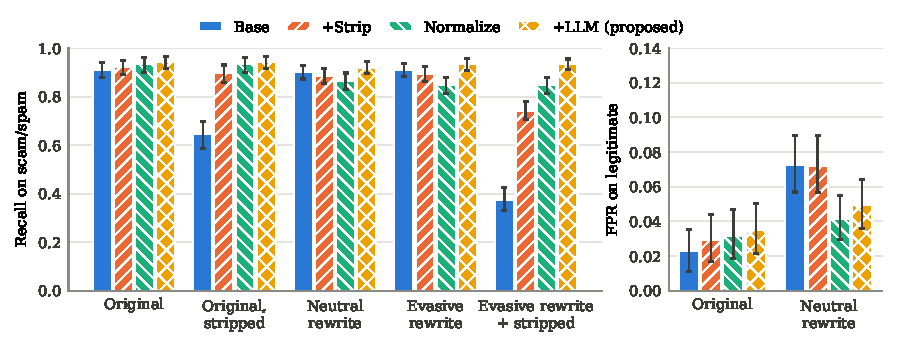
\includegraphics[width=\textwidth]{figures/recall_fpr.pdf}
\caption{TF-IDF recall under each attack (left) and false-positive rate (FPR) on legitimate messages (right), pooled over the three rewriting LLMs and five seeds. Error bars are 95\% bootstrap confidence intervals. Hatching distinguishes the training regimes in grayscale print. Table~\ref{tab:main} gives the values per LLM.}
\label{fig:main}
\end{figure}

Figure~\ref{fig:main} summarizes the TF-IDF results, and Table~\ref{tab:main} breaks them down by LLM. Rewriting alone has a small effect. With diacritics kept, the Base filter's recall on rewrites is 0.85--0.94, against 0.91 on the originals. This holds even for the evasive prompt. Diacritic stripping alone lowers recall to 0.65. A likely reason is that diacritic-free text is much more frequent among legitimate messages (61\%) than among scam/spam (34\%), so the Base filter learns to treat missing diacritics as a sign of legitimacy. Stripping correspondingly lowers its FPR on legitimate messages (0.012 versus 0.023). The combination is far stronger than either attack: evasive rewriting followed by stripping lowers recall to 0.48 (Qwen), 0.36 (NeMo) and 0.26 (SeaLLMs). SeaLLMs, the model tuned for Southeast Asian languages, produces the most damaging rewrites. This ranking persists after removing meaning-drifted rewrites (Section~\ref{sec:sens}).

Table~\ref{tab:style} supports this explanation by splitting recall by the diacritic style of the \emph{source} message. For the Base filter, scams originally written with diacritics are caught 97\% of the time, but only 56\% once their diacritics are stripped. Scams that were already diacritic-free are, as expected, unaffected by stripping (0.81 in both cases), and are harder to catch to begin with. The +LLM defense removes this asymmetry for diacritic-bearing sources (0.97 before and after stripping) and also raises recall on diacritic-free sources from 0.81 to 0.89.

\begin{table}[t]
\centering
\caption{TF-IDF recall split by whether the source scam/spam message was written with diacritics (5 seeds, mean). About two thirds of positive messages carry diacritics.}
\label{tab:style}
\small
\begin{tabular}{lcccc}
\toprule
 & \multicolumn{2}{c}{Base} & \multicolumn{2}{c}{+LLM (leave-one-out)} \\
\cmidrule(lr){2-3}\cmidrule(lr){4-5}
Test set & With diacritics & Without & With diacritics & Without \\
\midrule
\inputtable tables/by_source_style.tex
\bottomrule
\end{tabular}
\end{table}

\begin{table}[t]
\centering
\caption{TF-IDF results (5 seeds pooled, 95\% bootstrap CI in brackets). \emph{Neutral} and \emph{evasive} are LLM rewrites with diacritics kept as generated. \emph{+ stripped} removes diacritics after rewriting.}
\label{tab:main}
\small
\begin{tabular}{lcccc}
\toprule
Test set & Base & +Strip & Normalize & +LLM (leave-one-out) \\
\midrule
\inputtable tables/tfidf_main.tex
\bottomrule
\end{tabular}
\end{table}

\subsection{RQ2: false alarms on LLM-written legitimate messages}
Rewriting legitimate messages raises the Base filter's FPR from 0.023 to 0.039 (Qwen), 0.072 (NeMo) and 0.101 (SeaLLMs). The confidence intervals for NeMo and SeaLLMs do not overlap with the original. This suggests that a filter tuned on human-written traffic partly treats ``machine-like'' style as a scam cue. This matters as legitimate senders increasingly draft notifications with LLMs. No prior scam benchmark we are aware of measures this effect.

\subsection{RQ3: a lightweight defense}
Normalization alone removes the stripping attack but lowers recall on SeaLLMs rewrites to 0.74--0.80. Adding rewrites from the two \emph{other} LLMs fixes this. +LLM keeps recall at 0.85--0.96 under every attack, including the unseen rewriting model. On rewrites followed by stripping it improves recall over Base by 0.41--0.65 (paired bootstrap; all CIs exclude 0). On original messages it also improves recall by 0.033 (CI [0.008, 0.061]). Its FPR rises from 0.023 to 0.035 on original legitimate messages. On rewritten legitimate messages its FPR is lower than Base for NeMo and SeaLLMs (0.049 and 0.054 versus 0.072 and 0.101) and similar for Qwen (0.044 versus 0.039).

\subsection{TF-IDF versus PhoBERT}
Table~\ref{tab:phobert} compares the two detector families on the first three seeds. Base PhoBERT has a lower FPR on original messages (0.007) but is \emph{less} robust to rewriting than TF-IDF: its recall on SeaLLMs neutral rewrites is 0.74, against 0.88 for TF-IDF on the same seeds, and its FPR on rewritten legitimate messages rises up to ninefold. Augmentation helps PhoBERT in the same way it helps TF-IDF. PhoBERT +LLM is the most accurate configuration overall: recall 0.94 with an FPR of 0.015 on original messages, recall 0.88--0.97 under every attack, and an FPR of 0.017--0.046 on rewritten legitimate messages.

\begin{table}[t]
\centering
\caption{TF-IDF versus PhoBERT (seeds 0--2, mean $\pm$ s.d. over seeds). The first eight rows are recall; the last four are FPR.}
\label{tab:phobert}
\small
\begin{tabular}{lccccc}
\toprule
 & \multicolumn{2}{c}{TF-IDF} & \multicolumn{3}{c}{PhoBERT} \\
\cmidrule(lr){2-3}\cmidrule(lr){4-6}
Test set & Base & +LLM & Base & +Strip & +LLM \\
\midrule
\inputtable tables/phobert.tex
\bottomrule
\end{tabular}
\end{table}

\subsection{Deployment cost}
Table~\ref{tab:eff} reports model size and single-message CPU latency (batch size 1, one thread). The proposed TF-IDF filter, trained on all original and rewritten messages, needs 5.5\,MB and 1.6\,ms per message, small enough for on-device or gateway deployment. PhoBERT is about 100 times larger and slower (515\,MB, 170\,ms). It therefore buys its extra accuracy at a cost that matters for high-volume SMS gateways and on-device filtering. A dynamically quantized INT8 PhoBERT produced degenerate predictions in our environment, so we do not report it.

\begin{table}[t]
\centering
\caption{Model size and CPU latency per message (batch size 1, single thread). The TF-IDF model was measured on an Intel desktop CPU and PhoBERT on a Kaggle CPU, so the latencies are indicative only.}
\label{tab:eff}
\small
\begin{tabular}{lrrr}
\toprule
Model & Size (MB) & Mean (ms) & p95 (ms) \\
\midrule
\inputtable tables/efficiency.tex
\bottomrule
\end{tabular}
\end{table}

\subsection{Sensitivity to meaning drift}\label{sec:sens}
A rewrite that changes the meaning of a scam may stop being a scam. We therefore repeat the TF-IDF analysis after also removing rewrites with LaBSE similarity below 0.7. All conclusions hold. Base recall on evasive rewrites with stripping is 0.20--0.44. +LLM recall is 0.92--0.94. The Base FPR on rewritten legitimate messages is 0.040--0.075, against 0.036--0.039 for +LLM.

\section{DISCUSSION AND LIMITATIONS}\label{sec:disc}
Our results suggest that, for Vietnamese SMS, the cheapest attack, diacritic stripping, does far more damage than LLM paraphrase, and that defenders should normalize diacritics before worrying about paraphrase. The two attacks compound, and augmenting with rewrites from a \emph{different} LLM transfers to an unseen one.

The study has several limitations. The positive class mixes spam and scam. Test splits are small, which we address with confidence intervals but which still limits fine-grained comparisons. We use three open 7--12B LLMs with a single sampling configuration and no attacker who adaptively queries the filter. All messages come from a single public collection, so the findings may not cover other senders, periods or regions.
LLMs did not follow the instruction to keep the diacritic style. For this reason we report the stripped variants explicitly rather than relying on the generated style.

\textbf{Ethics.} We generate rewrites of \emph{existing} messages only to measure and improve detection. We release prompts and rewrites only for defensive research, and personal data in the source messages is already masked with placeholders.

\section{CONCLUSIONS}\label{sec:concl}
We introduced a controlled benchmark of LLM-rewritten Vietnamese SMS and showed that diacritic stripping, not paraphrase, is the dominant weakness of current filters. The two attacks compound to reduce recall by up to 65 points, and LLM-written legitimate messages are falsely flagged up to four times more often. A 5.5\,MB TF-IDF filter with diacritic normalization and leave-one-LLM-out rewrite augmentation keeps recall at 0.85--0.96 under every attack we tested. Future work includes adaptive attackers, larger and more recent message collections, and separating spam from scam.

\renewcommand{\refname}{\normalfont\fontsize{12}{14}\bfseries\filcenter REFERENCES}
\bibliographystyle{IEEEtran}
\bibliography{refs}

\end{document}
